%!TEX root = thesis.tex
\section{Key Expansion}
\label{ch:key_expansion}
The key expansion is defined in the \lstinline{key_expansion.py} file. It provides all the functions necessary to compute all round-keys. It was implemented jointly between the authors. It is written in python as it only needs to be executed once at the start of the en- or decryption. Therefore time complexity was no concern here.

\subsection{Expand Key}
\label{ch:expand_key}
The main function  \lstinline{expand_key} takes a 16 byte key and expands it into the round-keys.

\textbf{Args:}
\begin{itemize}
  \item \lstinline{key} 16-byte long key as a hexadecimal string
\end{itemize}

\textbf{Returns:}
\begin{itemize}
  \item Bytearray of all round-keys in the correct order
\end{itemize}

\begin{figure}
\centering
  \begin{minipage}{.65\textwidth}
    \centering
    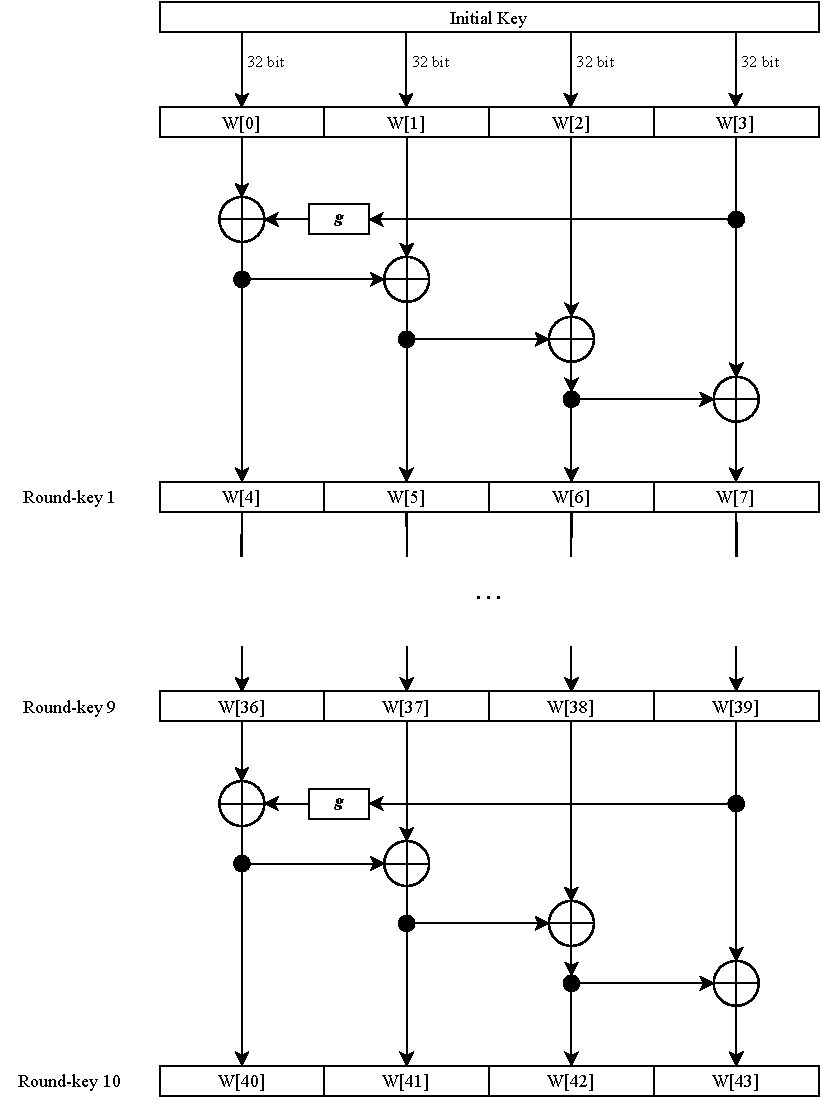
\includegraphics[width=\linewidth]{data/assets/key_expansion.pdf}
  \end{minipage}%
  \begin{minipage}{.35\textwidth}
    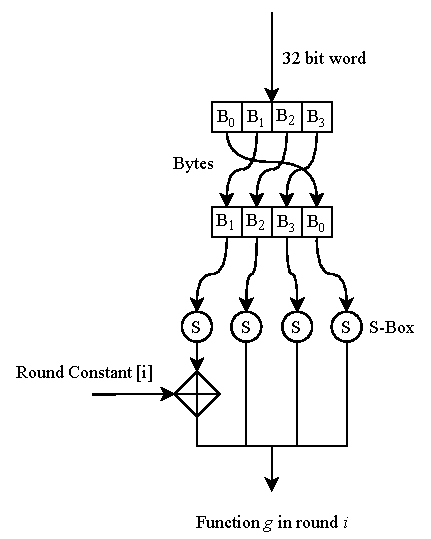
\includegraphics[width=\linewidth]{data/assets/g_function.pdf}
  \end{minipage}
  \caption{The key expansion algorith \cite{paar2016kryptografie}}
\end{figure}





\subsubsection{Order of Operations}
The input key is interpreted as hexadecimal and transformed into a bytearray. The bytearray is then split into 4-byte blocks, as most operations in the key expansion operate on 32-bit words. The round constants are computed via the  \lstinline{rcon_compute} function and stored in the  \lstinline{rcon} variable. The main part of the algorithm happens in a for-loop that counts from 4 to 43. The indices zero to three represent the initial key. For AES-128 there are ten round-keys plus the initial key. Represented in 32-bit words that makes 44 32-bit words. In the loop the first word of every key gets processed differently.

\subsection{Byte XOR}
\label{ch:byte_xor}
Function that uses the XOR operator or two bytes. This function is necessary because of how python represents bytes.

\textbf{Args:}
\begin{itemize}
  \item \lstinline{ba1} first byte of the XOR operation
  \item \lstinline{ba2} seconds byte of the XOR operation
\end{itemize}

\textbf{Returns:}
\begin{itemize}
  \item \lstinline{ba1 ^ ba2}
\end{itemize}

The operation is implemented by manually executing XOR one bit at a time:
\begin{lstlisting}
return bytes([a ^ b for a, b in zip(ba1, ba2)])
\end{lstlisting}


\subsection{Function G}
\label{ch:func_g}

The function \lstinline{g} rotates the four bytes it is given, substitutes each byte with the SBox and adds the round constant for the current round.

\textbf{Args:}
\begin{itemize}
  \item \lstinline{word} 32-bit input word representing four bytes
  \item \lstinline{round} current round index
  \item \lstinline{rcons} list of the round constants
\end{itemize}

\textbf{Returns:}
\begin{itemize}
  \item 32-bit word
\end{itemize}

\begin{lstlisting}
def g(word, round, rcons):
    # Rotate input word
    subword = bytearray(word[1:] + word[0:1])

    # S-Box substitution
    for idx, v in enumerate(subword):
        subword[idx] = sbox[v]

    # add round constant
    subword[0] = subword[0] ^ rcons[round]

    return bytes(subword)
\end{lstlisting}


\subsection{Round Constant Computation}
The formula for the round constant in round i is  \lstinline{2^i-1} in GF(128). The irreducible polynomial to get back into the finite field after multiplications is represented as  \lstinline{0b100011011} or  \lstinline{0x11b} or  \lstinline{283}.

For numbers larger than 255 (0xff) the result of a bit shift by one (representing times two in binary) would overflow into 9-bits. In these cases the resulting number XOR the irreducible polynomial shifted by as many bits as the number is over 8 will result in a number in the finite field.

\begin{lstlisting}
return [
    0x01 << i
    if 0x01 << i < 0xff
    else 0x01 << i ^ (0x11b << i - 8)
    for i in range(10)
]
\end{lstlisting}

The function returns the following values:
 \lstinline{[0x01,0x02,0x04,0x08,0x10,0x20,0x40,0x80,0x1B,0x36]}

\textbf{Args:}
\begin{itemize}
  \item None
\end{itemize}

\textbf{Returns:}
\begin{itemize}
  \item List of integers representing the round constants
\end{itemize}

\subsection{Challenges and Alternative Implementation Strategies}
The main implementation challenge with the key expansion is the conversion between 16-byte keys, 32-bit or four-byte words, and single bytes. The first approach was to treat everything as integers as the handling of bytes is not as practical in python as it is in other languages. This approach included writing a function to split large numbers into a list of smaller numbers of some bit-length (chunksize):
\begin{lstlisting}
def separate_into_chunks(num, chunksize=8):
    compare_constant = 0x01 << chunksize
    if num < compare_constant:
        return [num]
    else:
        return separate_into_chunks(num >> chunksize, chunksize) + [num % compare_constant]
\end{lstlisting}
This recursive function take some number and bit shifts and separates it into chunks of the given size until the whole number is separated. The output from this function worked in most cases. The edge case for this implementation are leading zeroes. It does not preserve them, as they are represented as base-10 integers and not bytes. The solution was to switch the whole implementation to bytestrings and bytearrays, which made some new functions necessary. The XOR operation is not atomic with bytes in python, therefore it needed to be implemented.

Another challenge was the return type of the final key-array. The output needs to be passed to function written in C. Therefore we settled on a bytearray, as the ctypes library can handle them well. The bytearray consists out of the initial key concatenated with all the round-keys. This is the appropriate organization for the encryption with the decryption simply using it in reverse.
